








\ps{I'm thinking an intro to globular clusters, then to modelling GCs with discussion of binaries,
	then to observations of binaries in GC}

\section{Globular Clusters}

Globular clusters (GCs) are dense, spheroidal collection of stars bound by their own self-gravity.
GCs are found in most galaxies, with the Milky Way hosting roughly 150, mostly located in the outer
halo. GCs typically represent some of the oldest stellar populations in the universe and are usually
in excess of 10 billion years old. Globular clusters were thought to have formed from a single giant
molecular cloud, resulting in a single coeval population of star with identical abundances. While
modern observation shave revealed that many clusters in fact have multiple independent population
with difference elemental abundances, most globular clusters are still well-approximated by a single
simple stellar population.

The dynamics of a cluster are almost entirely described by the gravitational interactions between
object in the cluster.

Any nice review paper I can cite or something similar?

Mention mass segregation

\subsection{Binaries in Globular Clusters}

Mention why we expect binaries in GCs to be different from field binaries. (cite a field binary and GC binary paper here)

Some dynamical effects of binaries, mention that we're focusing on hard binaries that we can treat
as point masses, not so much the long-period binaries that provide significant energy through
hardening during interactions.

The most obvious way that binaries can affect the dynamic of a cluster is through three-body
interactions which eject a star at high velocities. \ps{Mention we expect these to have mostly
	slowed down by present day due to hard binaries only.}


The second way that binaries can impact the dynamics of a cluster is simply due to their higher mass
when compared to single stars. Because binaries are tightly bound, for all interaction except for
the very closest, they effectively act as a single point mass equal to the sum of each component's
mass. In this way, binaries can affect cluster dynamics in much the same way that a large population
of white dwarfs or neutron star would (see for example \citet{Kremer2021}) \ps{discuss what these
	effects would be}. Through simple two-body interactions with other cluster members, binaries will
begin to migrate to the central regions of the cluster due to mass segregation. This predicted
increase in binary fraction as you get closer to the centre of a cluster is also seen in
observations \ps{cite something here}.

Check some of those "Binary Burning" papers.

\subsection{Observations of Binary Stars in Globular Clusters}

\paragraph{}
In general, there are two methods used to detect binaries within globular clusters: high-precision
photometric observations and radial velocity surveys.

\paragraph{}
High-precision photometry can be used to detect binaries along the main sequence which have a
significant difference in the mass of their components ( typically these systems have a mass ratio,
$q$, larger than $0.5$). These systems will appear to be raised above the main-sequence when plotted
on a colour-magnitude diagram as their colour will match that of a typical main-sequence star
however their luminosity will be the sum of both components. Figure
\ref{fig:1/main_sequence_binaries} shows the main-sequence of the cluster NGC 2298, the binary stars
in this cluster are visible above the main-sequence according to their mass ratio.
\citet{Milone2012} performed high-precision photometry on several globular clusters using the Hubble
Space Telescope's (HST) Advanced Camera for Surveys and was able to place strong constraints on the
binary fraction for binaries with a mass ratio above $q=0.5$. This method allows for large studies
of binary populations in GCs without the need for dedicated observations but suffers from an
inherent bias towards systems with high mass ratios. Systems with mass ratios below $q=0.5$ are
typically too close to the regular main-sequence to confidently classify as binaries (see Figure
\ref{fig:1/main_sequence_binaries}). This means that studies which employ this method must assume an
underlying mass-ratio distribution if they wish to place any limits on the overall binary fraction
of a cluster.


\begin{figure}
	\centering
	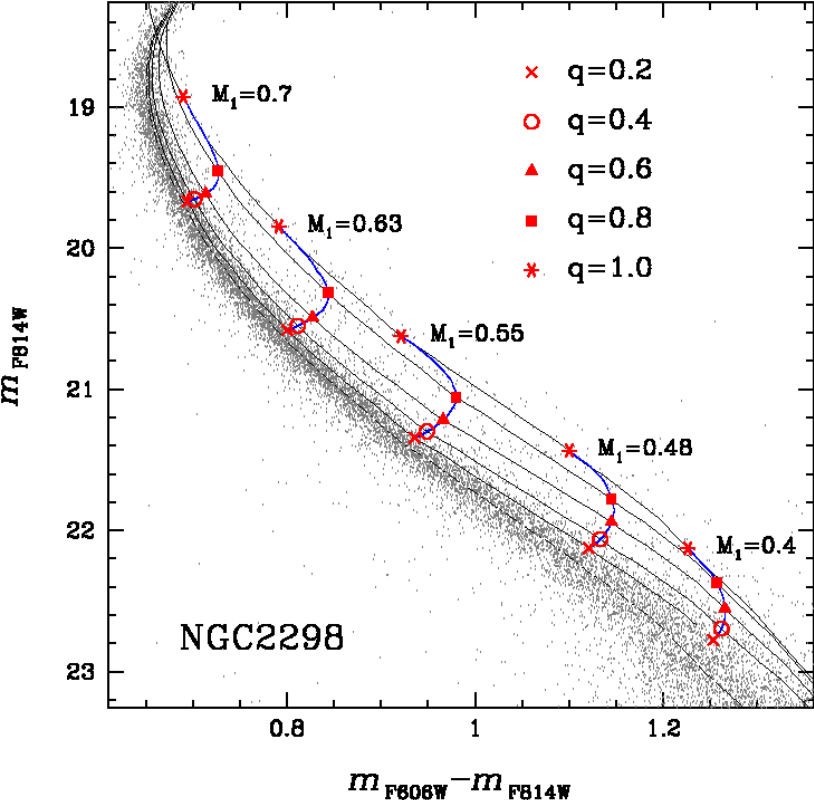
\includegraphics[width=0.8\textwidth]{"./figures/main_sequence_binaries.pdf"}
	\label{fig:1/main_sequence_binaries}
\caption{\ps{TODO: write proper caption} Reproduced from Figure 1 of \citet{Milone2012}.}
\end{figure}


Large-scale campaigns to measure the radial velocities for many stars in a cluster over several
epochs are another method which can be used to detect binaries in GCs. Systems which are found to
have periodically varying radial velocities can typically be confidently classified as binary
systems. \citet{Giesers2019} used the MUSE integral field spectrograph installed at the European
Southern Observatory's Very Large Telescope to observe several GCs and reported the results for NGC
3201. Integral field spectrographs provide spatially resolved spectra for the entire field of view
of the detector which enables far more time-efficient surveys than previous methods. Because this
methods measure radial velocities and periods, it can be used to constrain most of a binary system's
orbital parameters allowing us to verify our assumptions \ps{does it validate them? some binaries
	with periods up to 1000 days there?} about the period distributions of binaries in globular
clusters. \ps{grab a figure from the MUSE paper with period distribution?}



\section{Modelling Globular Clusters}

\paragraph{}
When modelling globular clusters, there are generally two approaches you can take. The first is to
model the entire evolutionary history of the cluster from initial conditions to the present. The
most commonly employed versions of these "evolutionary models" are direct N-body integration (see
for example \citet{Baumgardt2017a}) which directly calculate the gravitational interactions between
each object in the cluster and Monte-Carlo models (see \citet{Rodriguez2021} or \cite{Hypki2013})
which approximate the gravitational interactions between object according to the method of
\citet{Henon1971}. While these models provide insight into the dynamical history of the cluster,
they are very computationally expensive with even the fastest models taking on the order of a day
to model a realistic globular cluster \citep{Rodriguez2021}.

The second approach is to model just the present-day conditions of the cluster. These models, which
we call "equilibrium models", capture none of the dynamical history of the cluster but fully
describe the present-day state of the cluster and are orders of magnitude faster to compute with
typical models being on the order of a second. The comparative efficiency of these models enables
the use of statistical fitting techniques like MCMC or Nested Sampling which would be prohibitively
expensive to use with evolutionary models. This means that instead of a computing a grid of models
and finding the "best-fitting" model we can instead recover posterior distributions for key cluster
parameters.

In this work we use the \code{LIMEPY} family of models presented by \citet{Gieles2015}. \ps{Describe
	how the models work}. In their current implementation, these models assume that all objects
within the cluster are single and make no attempt to model the dynamical effects of stellar
multiplicity. In this project we adapt these models to incorporate some of the effects of
binary stars under the assumption that all long-period binaries have been ionized by the
present-day.